\section{Results}
Particularly Suicide watch community consists of over 78k subscribers and reader, however is supported by mere 12 Moderators according to the latest count. The moderators are mainly present to prevent any kind of abuse, trolling or non-clinical or non-productive advices \ns{What is the role of the moderators, ie how heavily is the forum moderate? And we need a date rather than latest count} These moderators are volunteers and do have a training, albeit through experience of interactions on the forum. \ns{Need citation that they have training through experience. I think you mean experience on the site}. All the moderators have been in that role for at least 3 years and the oldest goes as far as December 2008. 

Our study is based on all conversations on SuicideWatch, represented as user and reply graphs. \ns{These need to be defined before.}
Through our analysis we find several discriminatory factors among Suicide watch conversations and generic front page conversations. We show that some of these factors are predictive of suicide watch conversations to a very high degree. We also show that certain properties of these conversations can be backed by sociological theories of real life support conversations. 

\subsection{Qualitative Analysis}
\sv{To be filled in - what would be a good title?}

\subsection{Network Characterization}
We begin by characterizing the two networked abstractions, namely Reply Graphs and Interaction graphs as described in Section \ref{Sec:Reply_graphs} and Section \ref{Sec:Interaction_graphs}. We do so by first comparing these two abstractions with a baseline control conversation threads using certain macroscopic network properties. 
We look at two prime metrics, 1) Distribution of size of user graphs (number of nodes in the network)  2) Maximum Depth of a branches in the Reply graphs. 
Figure \ref{fig:depthDist} shows the distribution of maximum depths across all Reply graphs for SW and Baseline subreddits. The SW threads depths have a median depth of 2 and mean of 4 compared to median depth of 2 for BL and a mean of 2.5. This shows that statistically the depths of Suicide watch and baseline graphs are quite similar.

\begin{figure}[!ht]
	\centering
	% \hspace*{-5mm}
	\subfloat[]{
		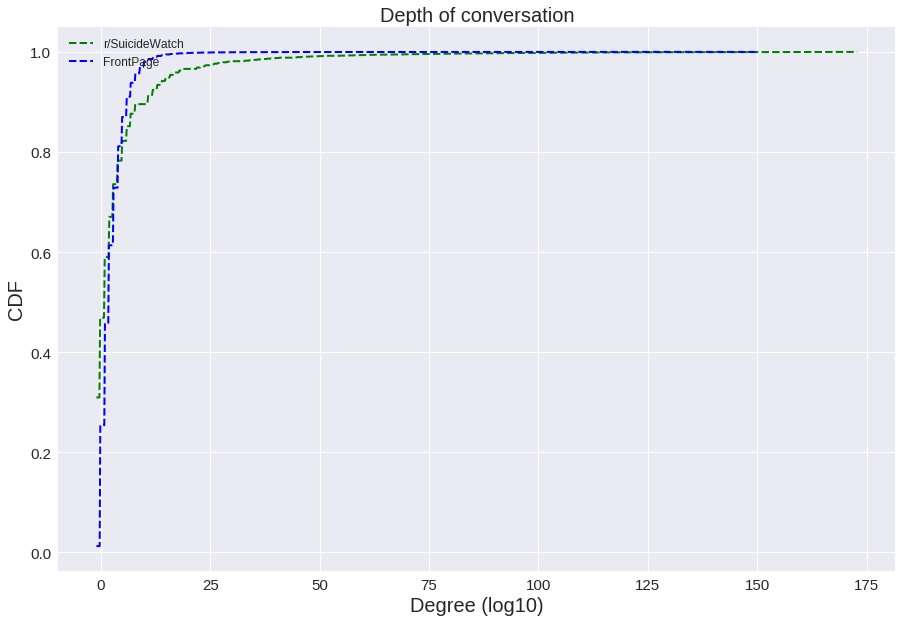
\includegraphics[width=0.4\textwidth, height = 5cm ]{Figures/DepthConversations.png}
		\label{fig:depthDist} }	
    \subfloat[]{
		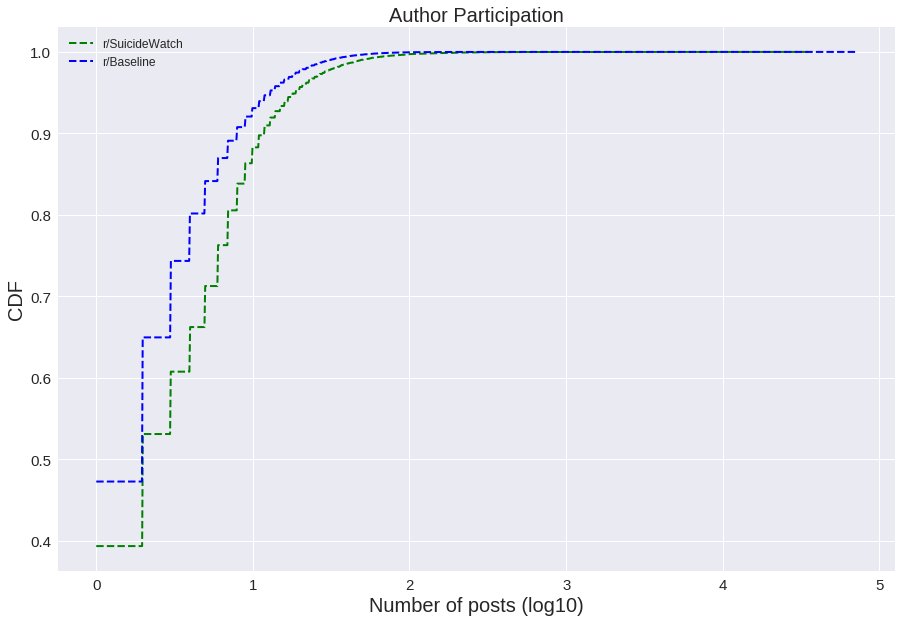
\includegraphics[width=0.4\linewidth, height = 5cm ]{Figures/AuthorParticipation.png}
		\label{fig:uniqAuthors}
	}
    
    
    \subfloat[]{
		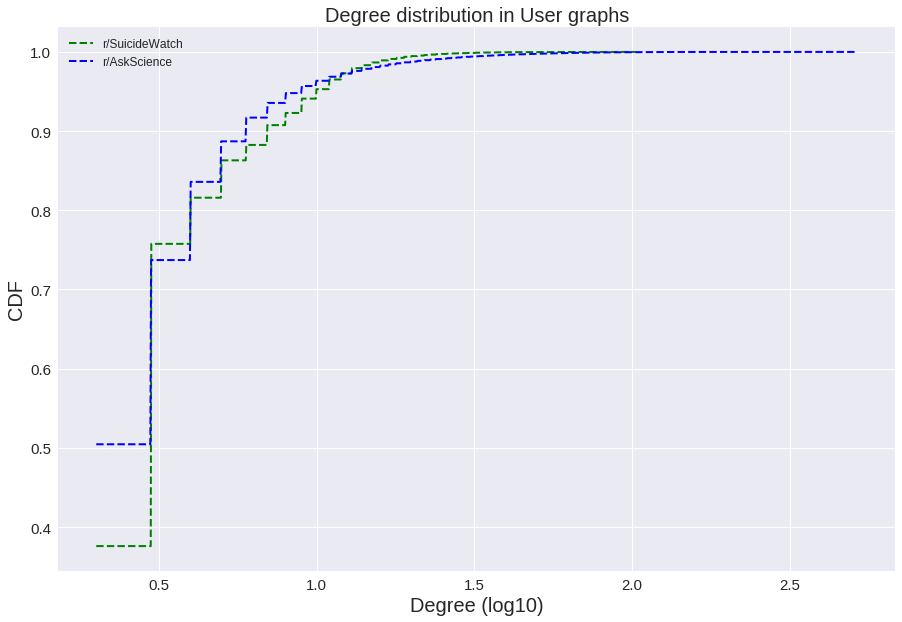
\includegraphics[width=0.4\textwidth, height = 5cm ]{Figures/degreeDistUgraph.png}
		\label{fig:degUgraph}
	}
	\subfloat[]{
		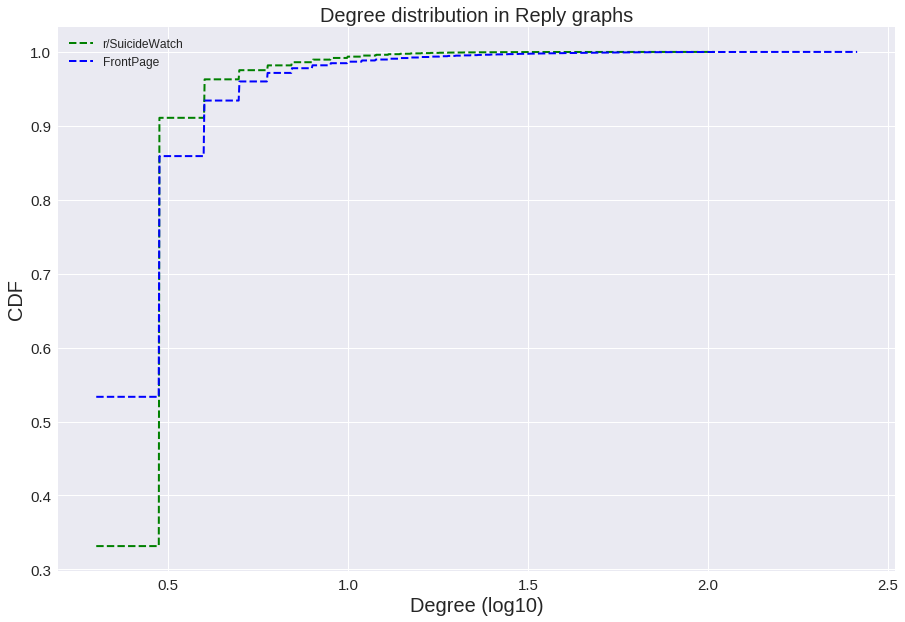
\includegraphics[width=0.4\linewidth, height = 5cm ]{Figures/degreeDistReplyGraph.png}
		\label{fig:degRgraph}
	}
\caption{\textsl{ Fig \ref{fig:depthDist} shows the distribution of maximum depths of Reply Graphs for Subreddit r/SuicideWatch and the baseline Frontpage conversations. Fig \ref{fig:uniqAuthors} shows the distribution of unique authors per thread in the two datasets. Fig \ref{fig:degRgraph} shows Distribution of degrees for Reply Graphs,  r/SuicideWatch and FrontPage. Fig \ref{fig:degUgraph} shows the degree distributions for the reply graphs}}
\end{figure}

However if we  compare the number of unique users per thread, the two communities exhibit considerable difference. SW subreddit has a median of 5 users per thread and a mean of 6.7 users and BL threads have a median of 25 users and mean of 50 unique users.
\remSVi{This might be better to present first in the results section (after the qualitative analysis)?}
Figures \ref{fig:degRgraph} and \ref{fig:degUgraph} show the comparison of degree distributions for both user and Reply graphs for SW and BL threads. Despite having differences in terms unique user participation, these two communities look very similar in terms of classical degree distribution metrics, which have been a standard goto measures for classifying networks \sj{cite}.

\subsection{How urgent are user responses?}
Understanding the inter message times can act as a good proxy for the urgency in a conversation. To understand how Suicide watch subreddit users responds to a $OP$ compared to other sub-reddit threads on the frontpage, we calculate differences between the posting times between consecutive messages in a reply graph. Figure \ref{fig:urgency} shows comparison using CDFs of inter-message response times for SW and FP threads. It can be seen that SW $OP$ are responded with the highest urgency amongst the 4, especially compared to either the $OP$ or any other users or sub-reddits. 

\begin{figure}[!ht]
	\centering
	% \hspace*{-5mm}
	\subfloat[]{
		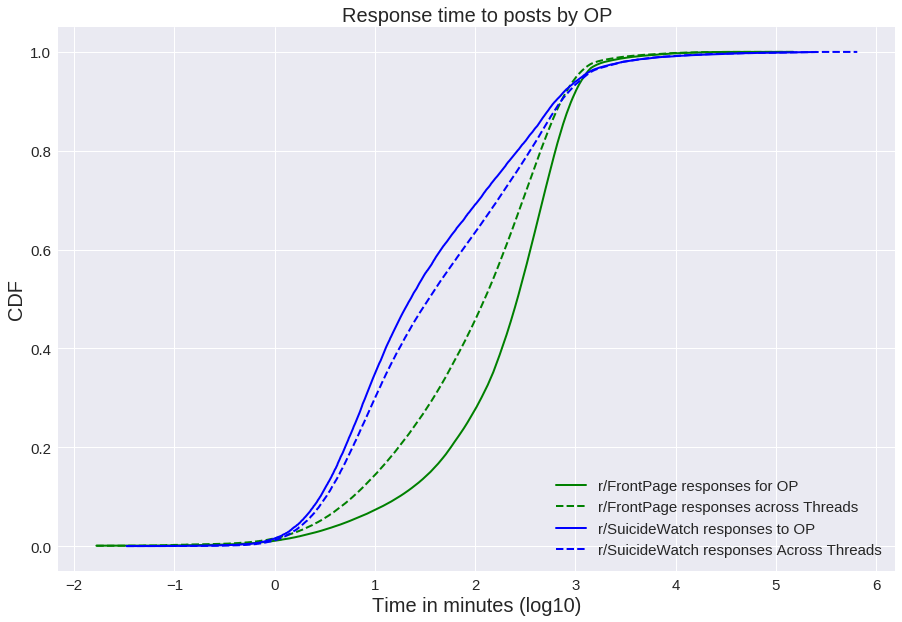
\includegraphics[width=0.45\textwidth, height = 5cm ]{Figures/respTimeDist.png}
		\label{fig:urgency}
	}
	\subfloat[]{
		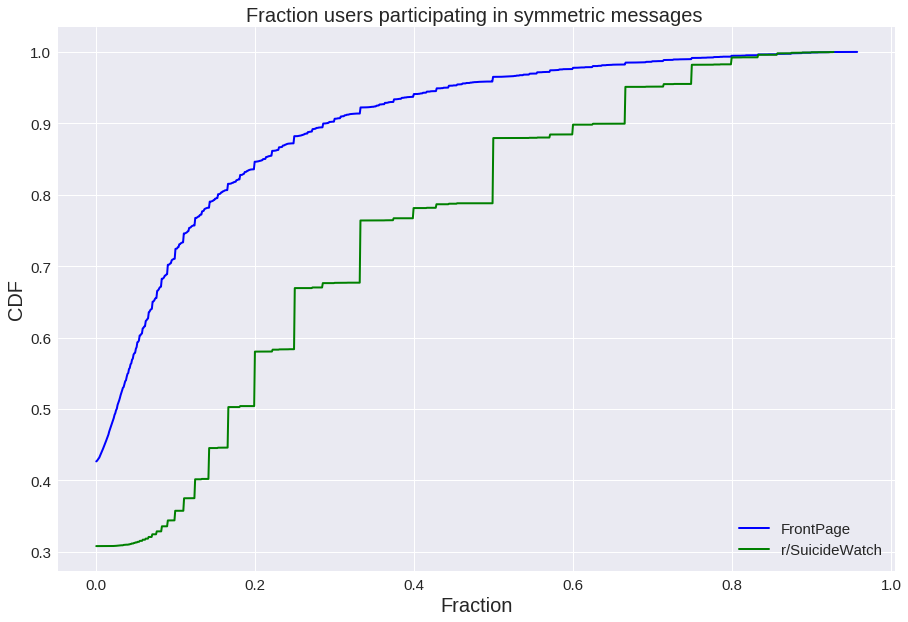
\includegraphics[width=0.45\linewidth, height = 5cm ]{Figures/SymUsers.png}
		\label{fig:sym}
	}
    
    \subfloat[]{
		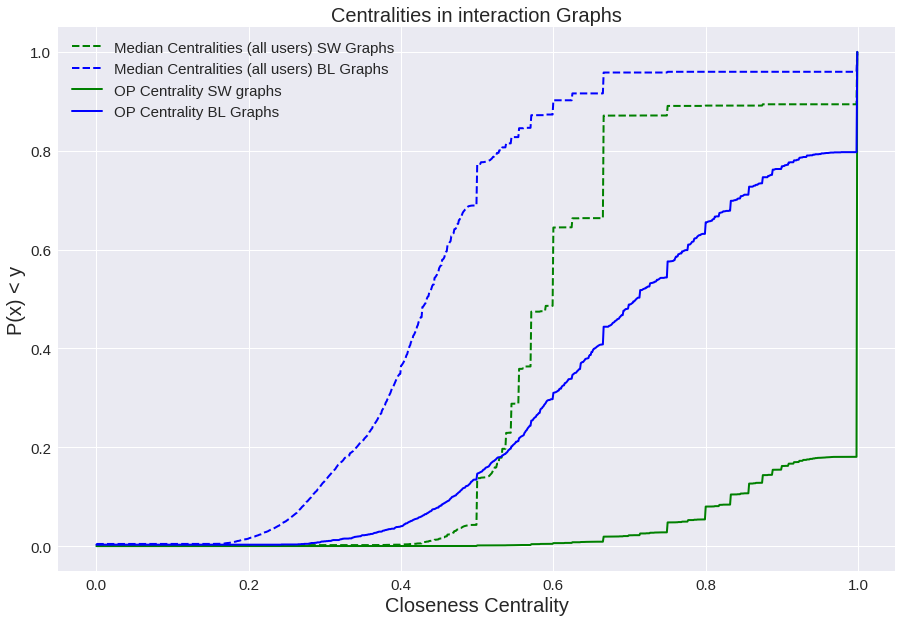
\includegraphics[width=0.45\linewidth, height = 5cm ]{Figures/AllCentralities.png}
		\label{fig:centrality}
	}
    \subfloat[]{
		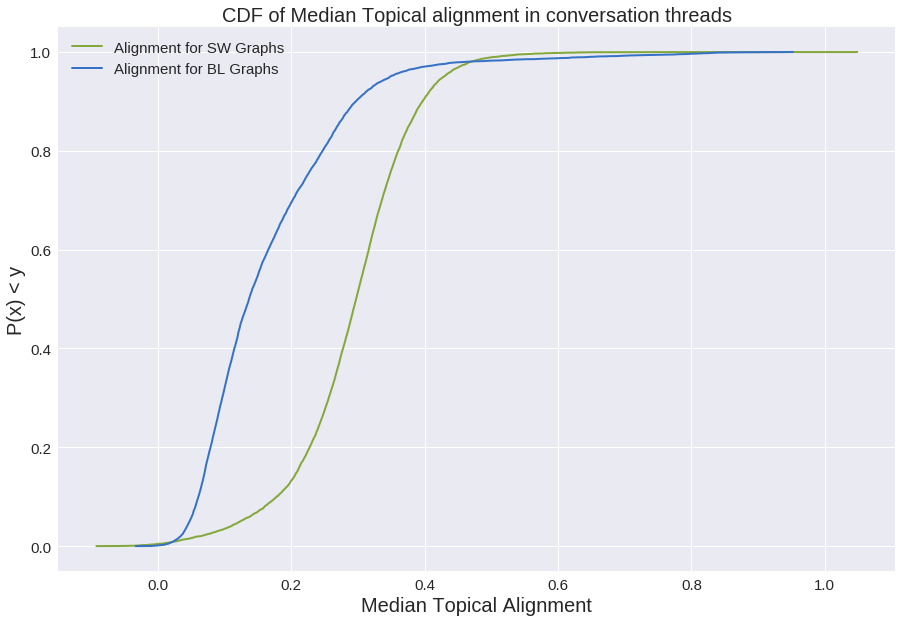
\includegraphics[width=0.45\linewidth, height = 5cm ]{Figures/medianTA.png}
		\label{fig:topical}
	}
    
    \subfloat[]{
		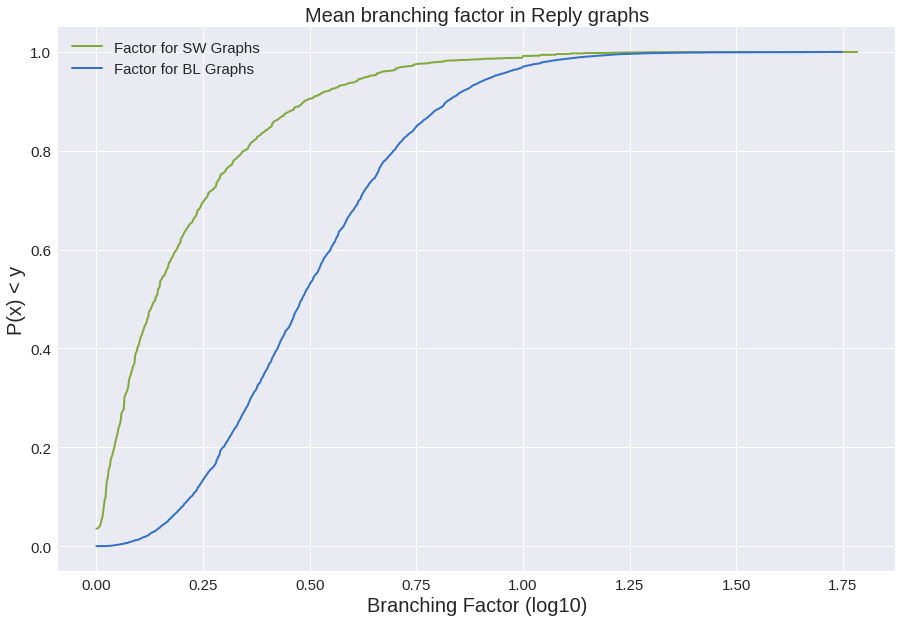
\includegraphics[width=0.45\linewidth, height = 5cm ]{Figures/meanBranchingFactor.png}
		\label{fig:branching}
	}
    \subfloat[]{
		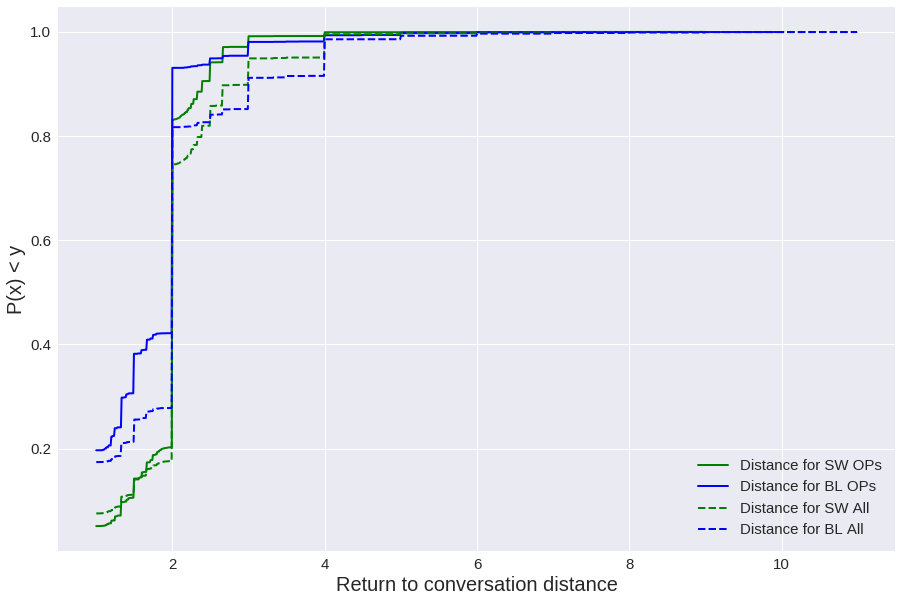
\includegraphics[width=0.45\linewidth, height = 5cm ]{Figures/returnDistance.png}
		\label{fig:returndist}
	}
    
    
\caption{Panel shows ECDFs of different network metrics. Fig.\ref{fig:urgency} shows the response time distributions, Fig.\ref{fig:sym} shows symmetrically engaged users, Fig.\ref{fig:topical} shows topical similarities across posts and \ref{fig:branching} shows the branching factors of reply graphs. }
\end{figure}

\subsection{How symmetric are the interactions?}
Despite signs of urgency and engagement, we ask the question: what percentage of conversations happening on these subreddits are symmetric in nature ? 
For this The median value for $U_{sym}$ for SW is 20\% where as for AS is 0\%. This shows that SW subreddit engages is a lot more symmetric conversation that the baseline threads.
If we define a set of users who engage in symmetric activity with the $OP$ , it would be worth while to investigate how much of the total message activity on the thread is carried out by these set of symmetric users . To calculate this we find the fraction of messages on each thread written as part of this symmetric conversation. Figure \ref{fig:sym} shows the trend. It can be see that SW threads contain a higher prevalence of symmetric message exchanges compared to the baseline Frontpage threads. This shows a higher engagement from the $OP$s side when participating in a supportive conversations

\subsection{How central are the users?}
To understand how embedded is the $OP$ in a conversation thread, we compare the betweenness centralities of $OPs$ in the $SW$ dataset with the baseline $FP$ dataset. 
Betweenness centrality is a good proxy of understanding how closely linked is a node with the rest of the network. When we calculate this metric for the user graphs we see that Suicide watch $OP$s tend to have highest centralities compared to generic $FP$ threads moth in terms of $OP$ centrality as well as median centrality across all the users. The high centrality of $OP$s in $SW$ conversations implies a high level of embedded-ness as well as a $OP$ centric approach by other participants in the conversation. The Figure \ref{fig:centrality} shows the Empirical CDFs of centralities. 

\subsection{How topically aligned are the responses?}
Topical alignment, or semantic symmetrically has been used as a measure of similarity between corpus of texts before\cite{Blei2003}


\subsection{How branched do conversations become?}
Branching in a conversation thread could be either a sign of digression or a sign interestingness resulting in more people joining in. To measure this phenomena, use the reply graphs, which resemble a n-ary directed acyclic graph, to evaluate the branching factor. 

\subsection{How often do users come back to respond ? }



\subsection{Are there any local interaction patterns?}
To answer this question, we use a method more commonly known as network motif analysis to understand triads, or groups of three nodes, and the patterns of edges that exist between them. 

\begin{figure}[!ht]
	\centering
	% \hspace*{-5mm}
% 	\subfloat[]{
% 		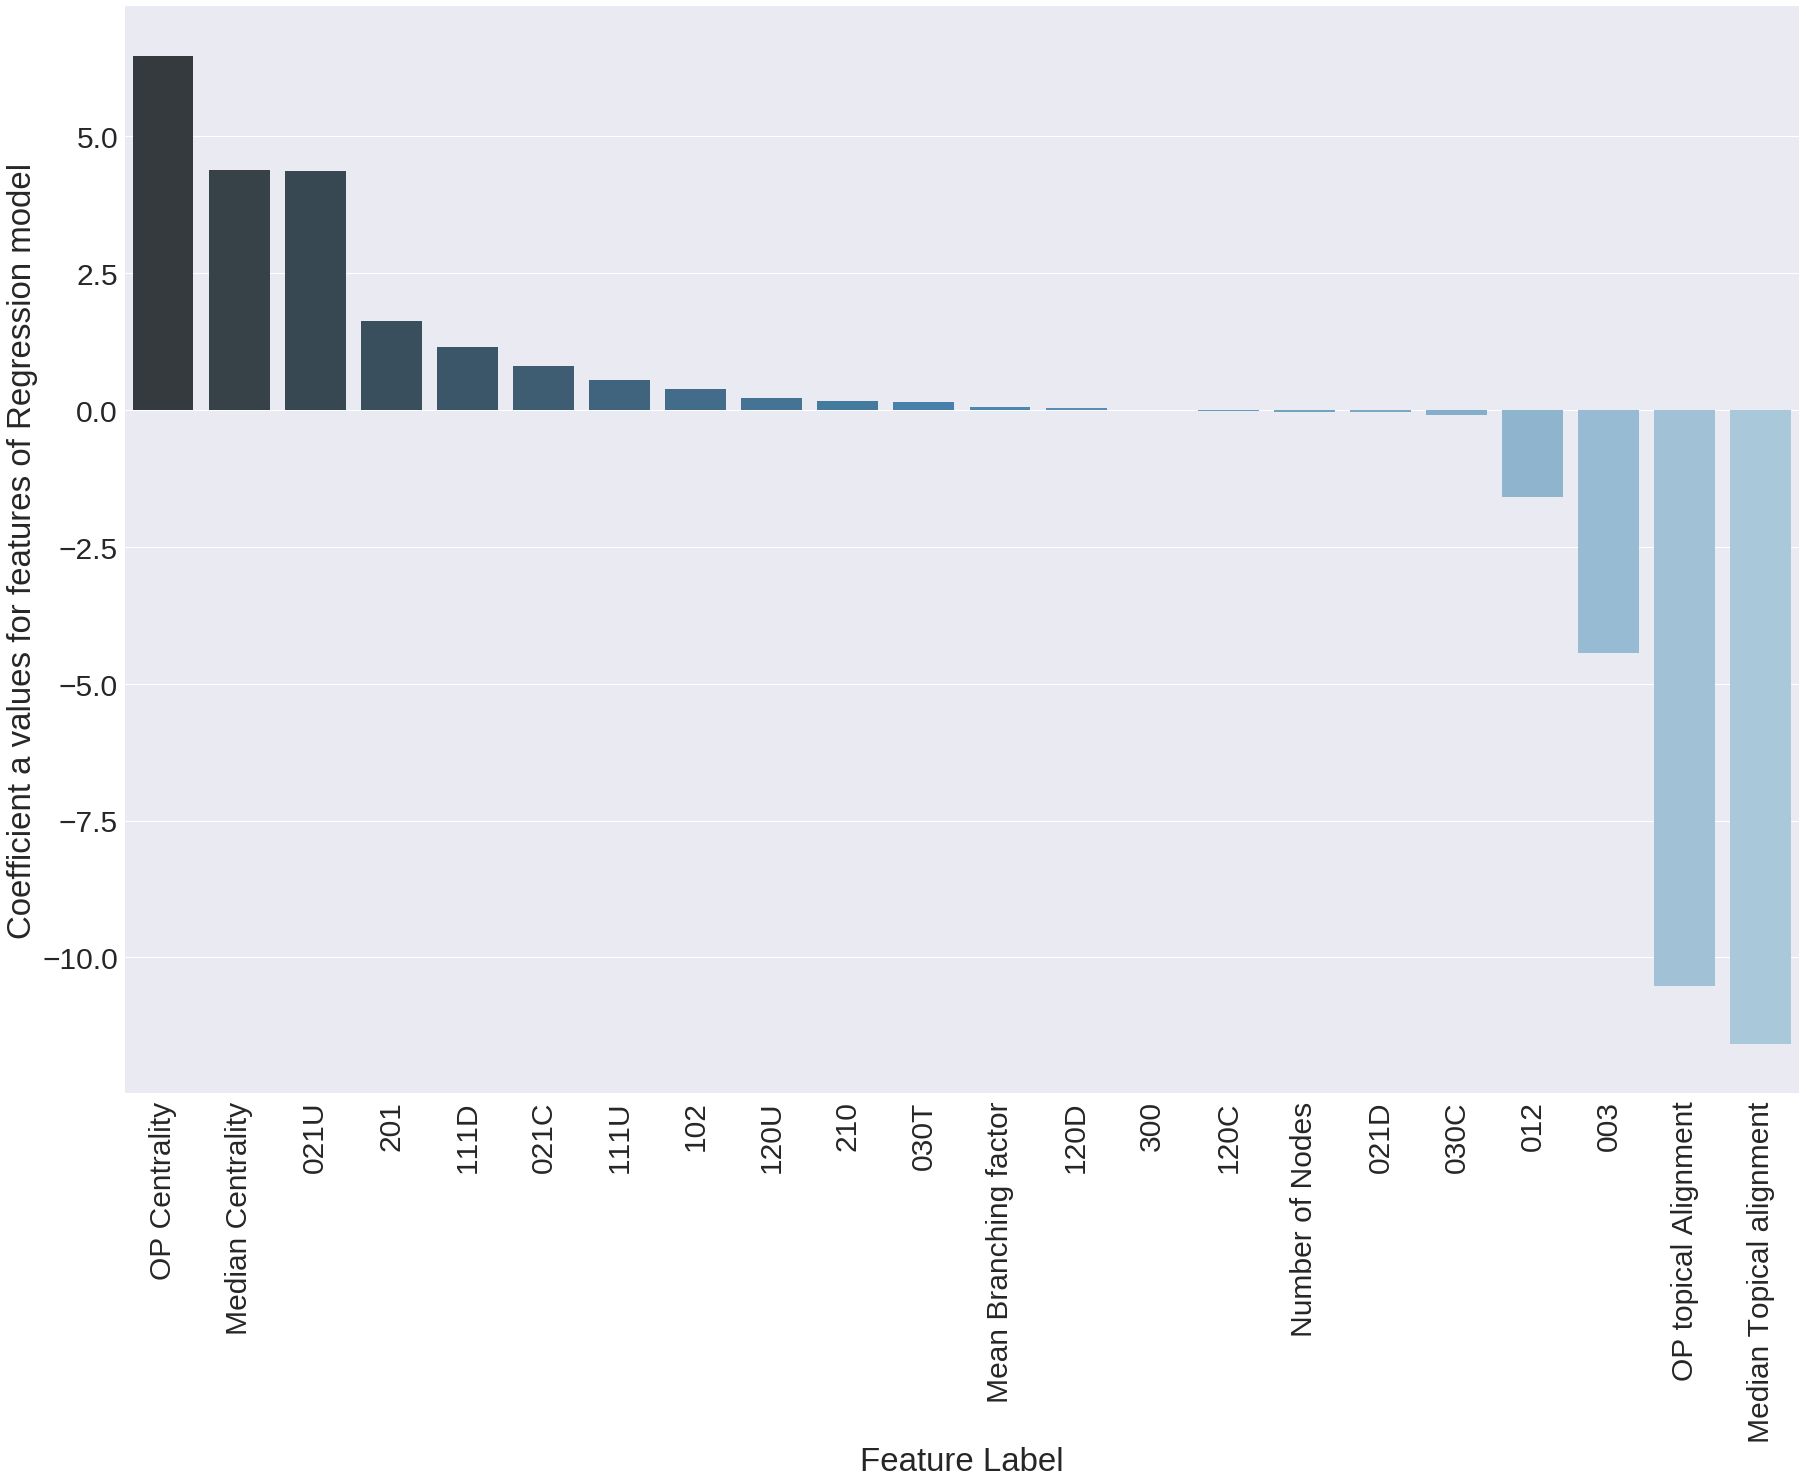
\includegraphics[width=0.5\textwidth, height = 6cm ]{Figures/RevisedFeatureRegression.png}
% 		\label{fig:feats}
% 	}
% 	\subfloat[]{
% 		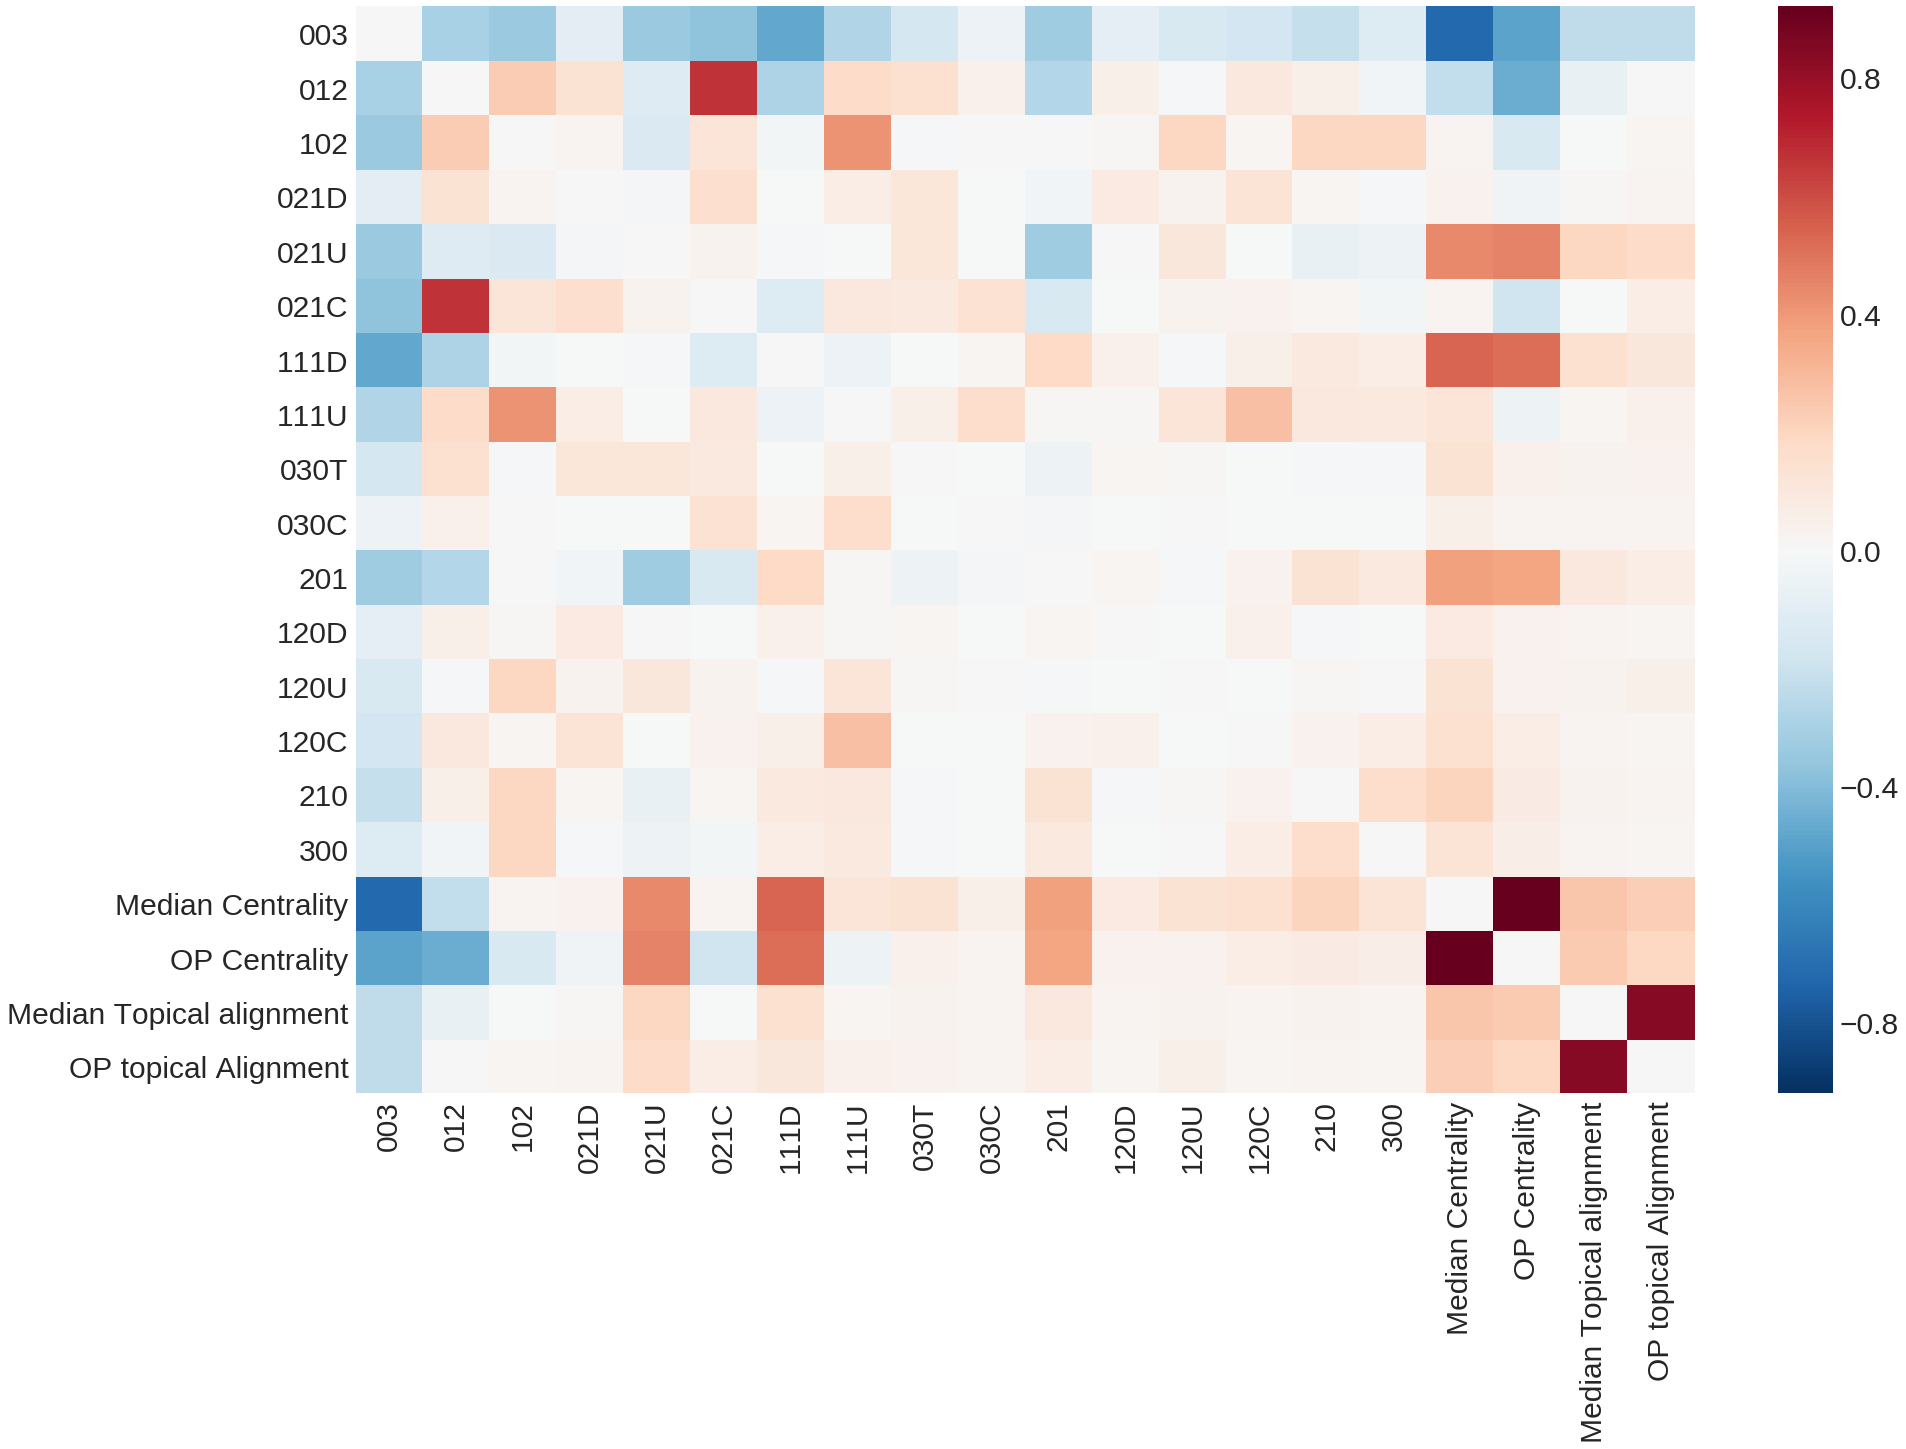
\includegraphics[width=0.5\linewidth, height = 6cm ]{Figures/normalized_corr.png}
% 		\label{fig:corrs}
% 	}
    
    \subfloat[]{
		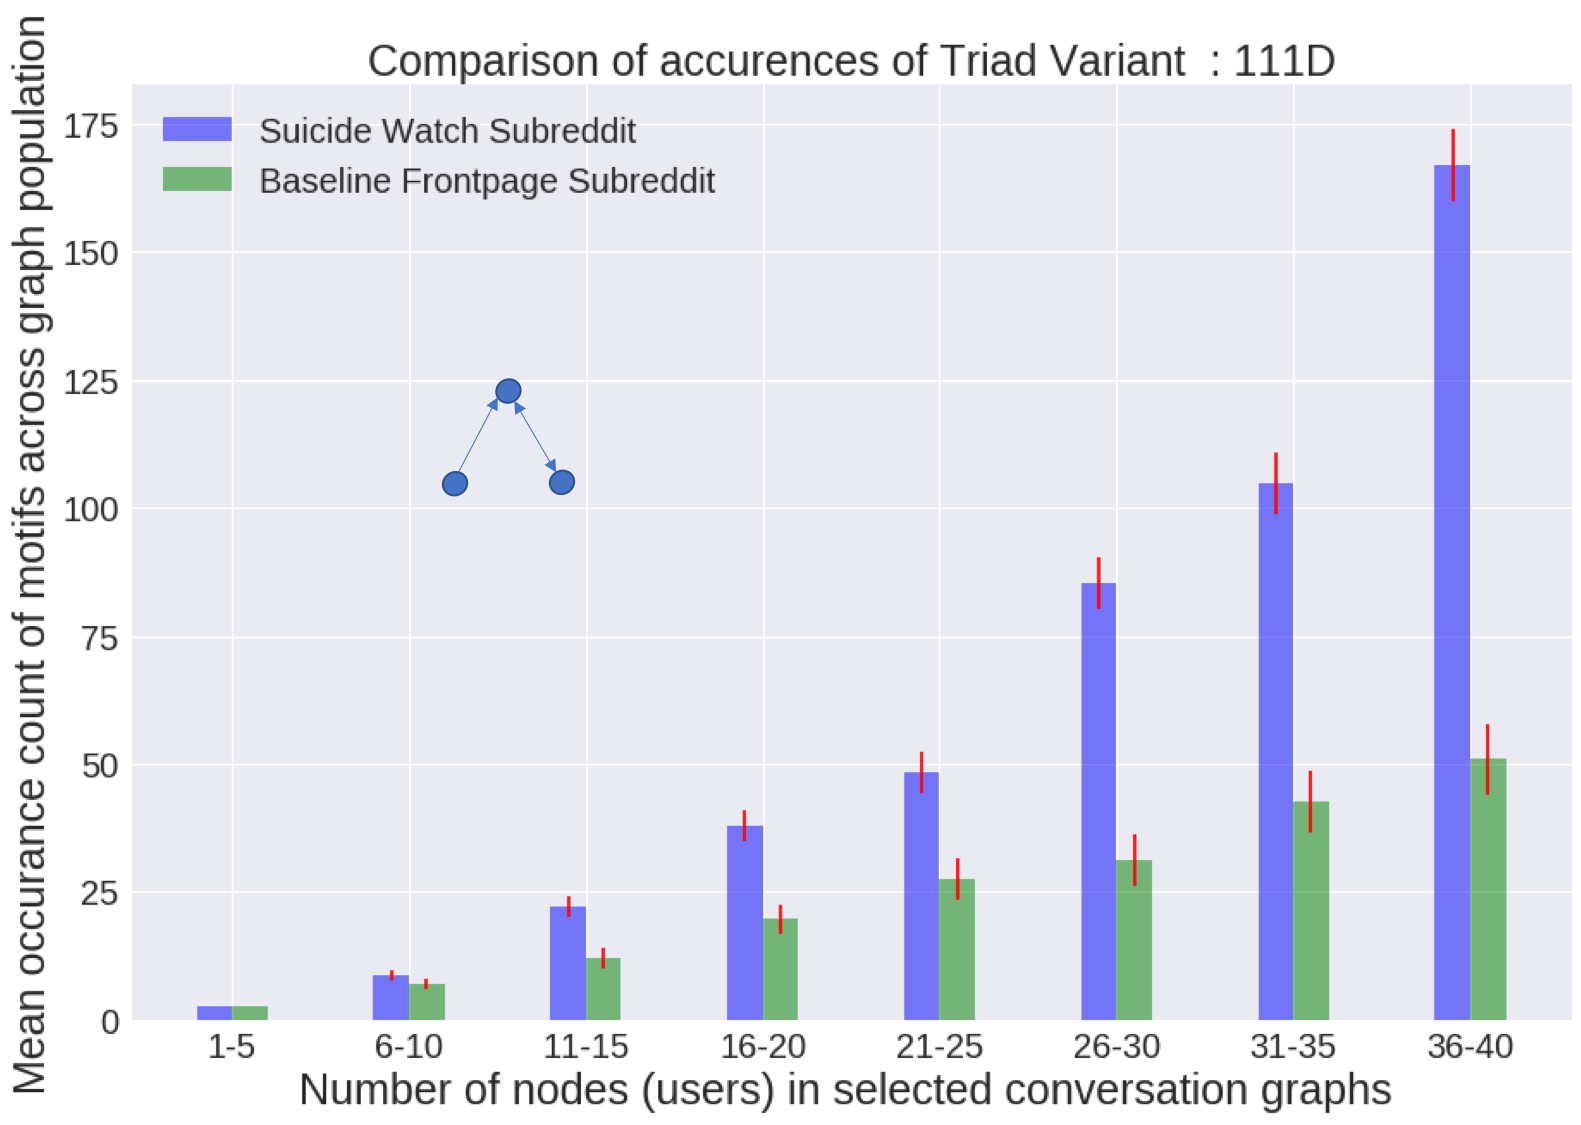
\includegraphics[width=0.5\linewidth, height = 6cm ]{Figures/111D.png}
		\label{fig:111D_over}
	}
    \subfloat[]{
		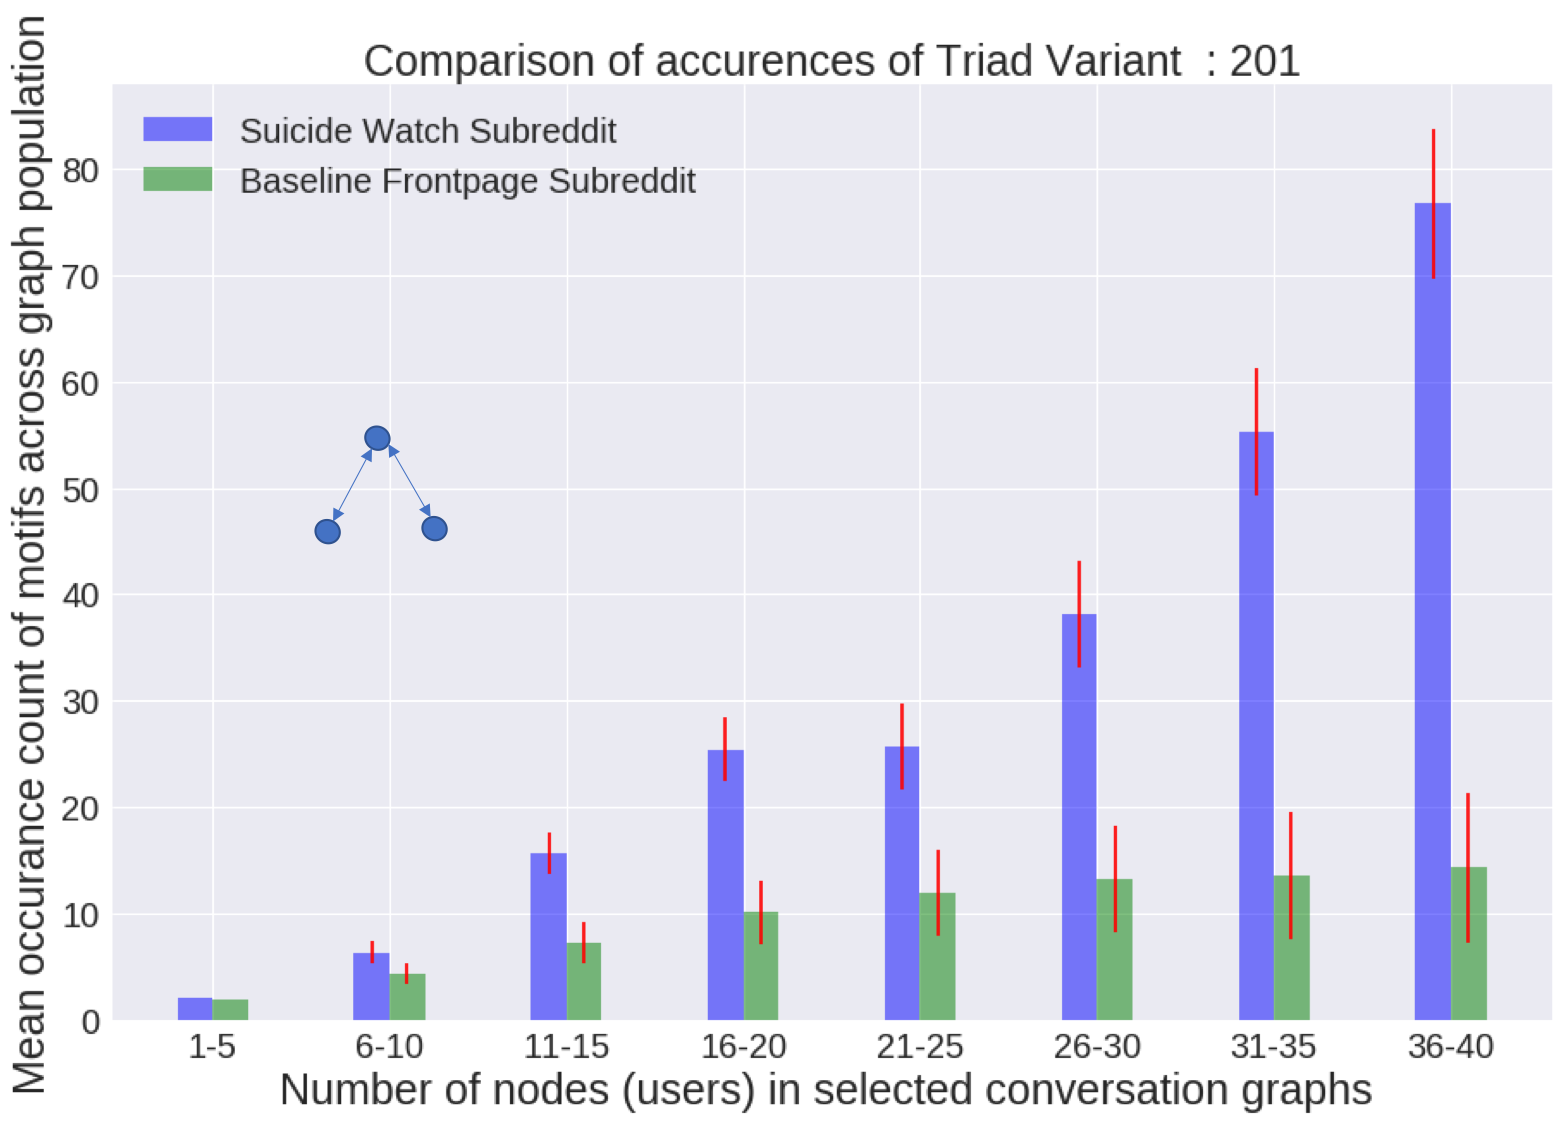
\includegraphics[width=0.5\linewidth, height = 6cm ]{Figures/201.png}
		\label{fig:201_over}
	}
    
    \subfloat[]{
		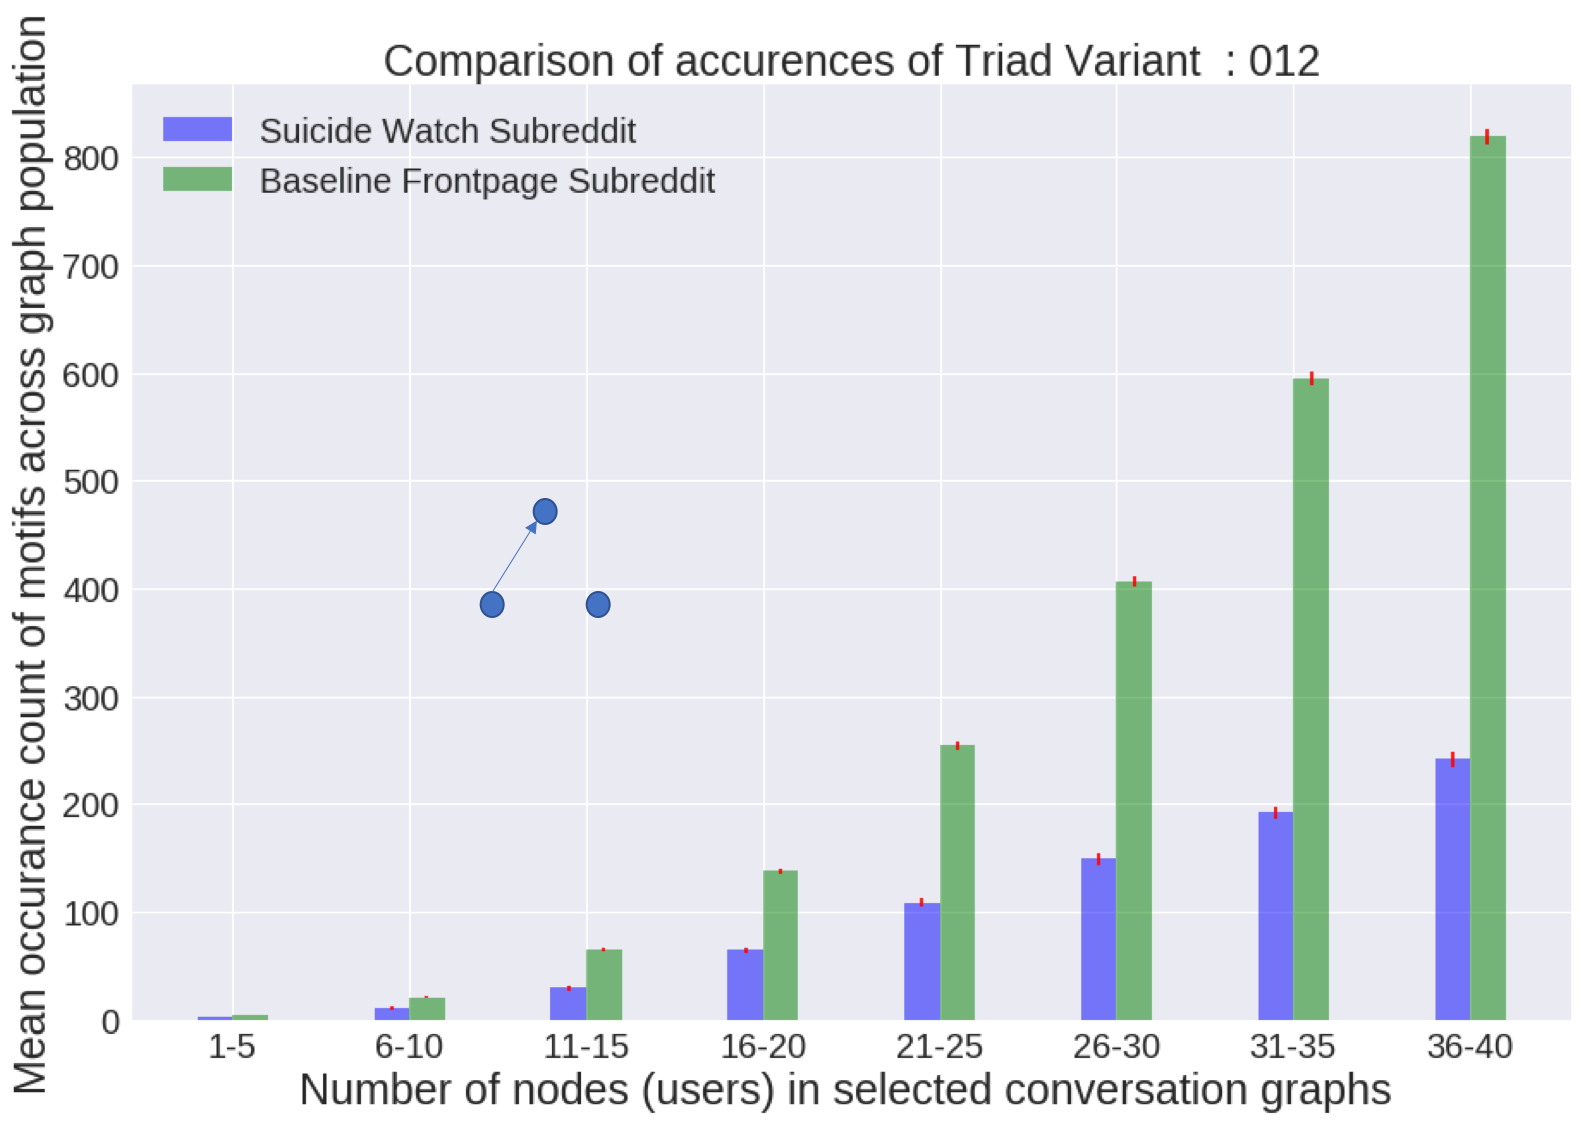
\includegraphics[width=0.5\linewidth, height = 6cm ]{Figures/012.png}
		\label{fig:012_over}
	}
    \subfloat[]{
		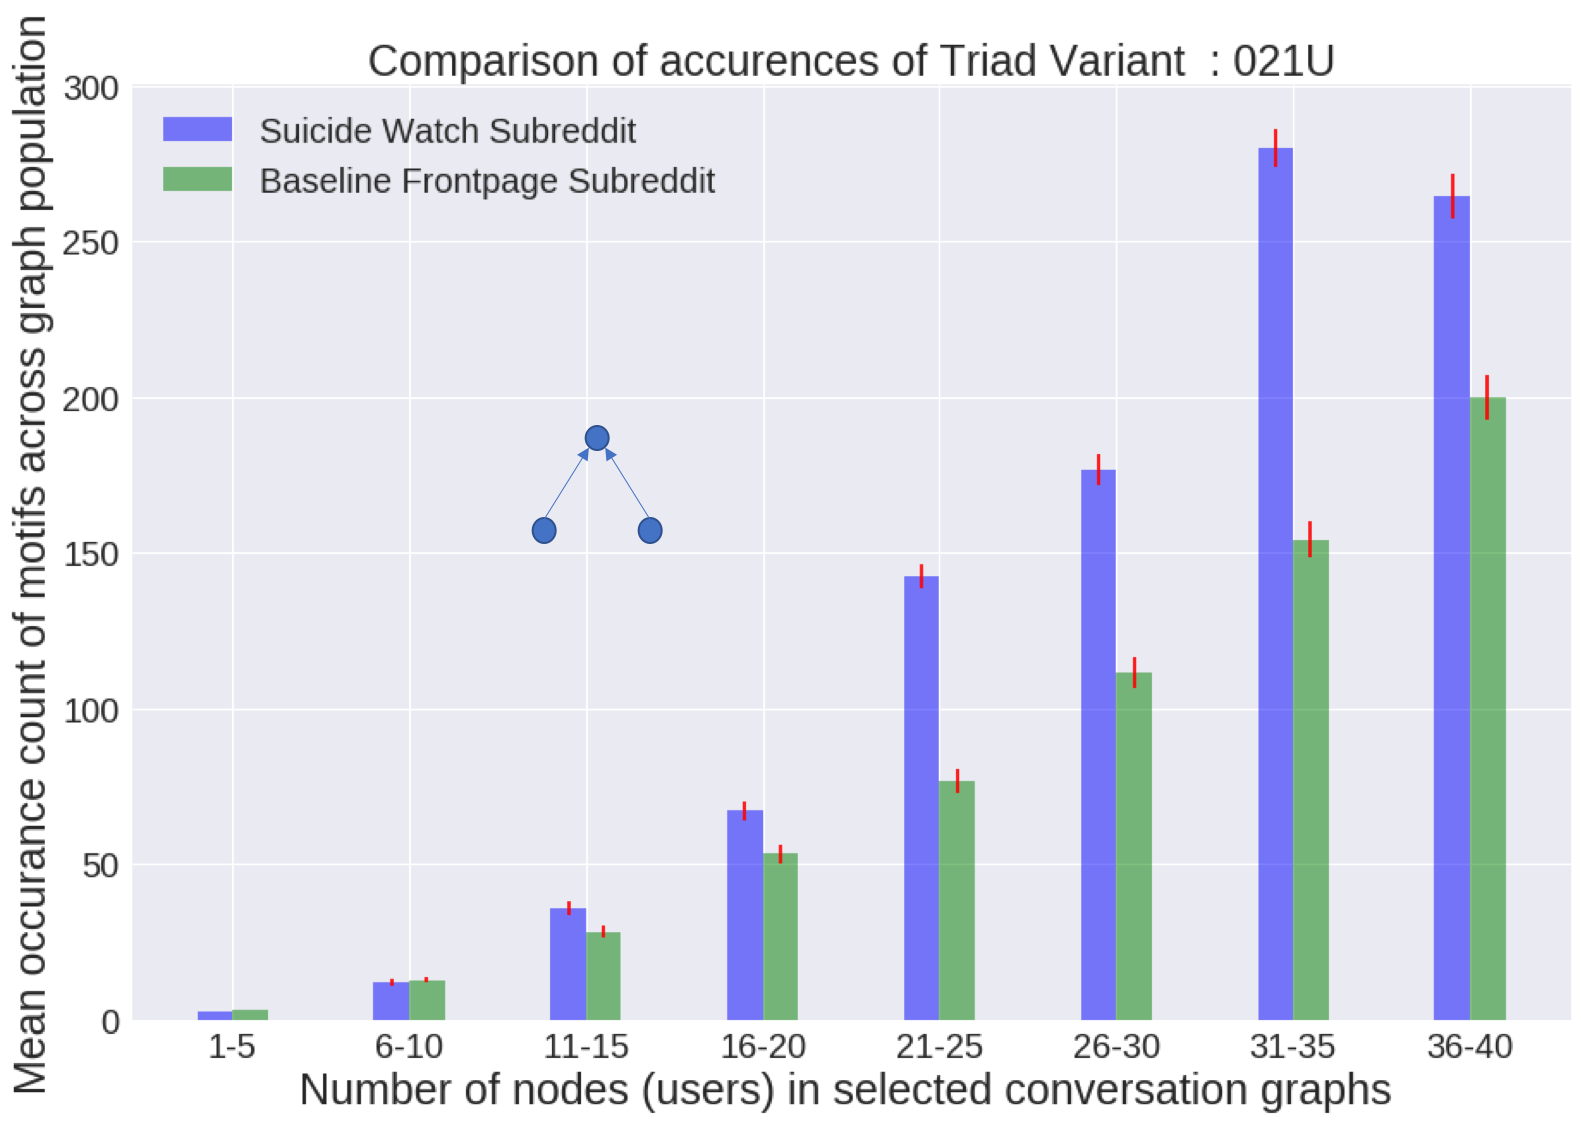
\includegraphics[width=0.5\linewidth, height = 6cm ]{Figures/021U.png}
		\label{fig:021U_over}
	}
    
    \subfloat[]{
		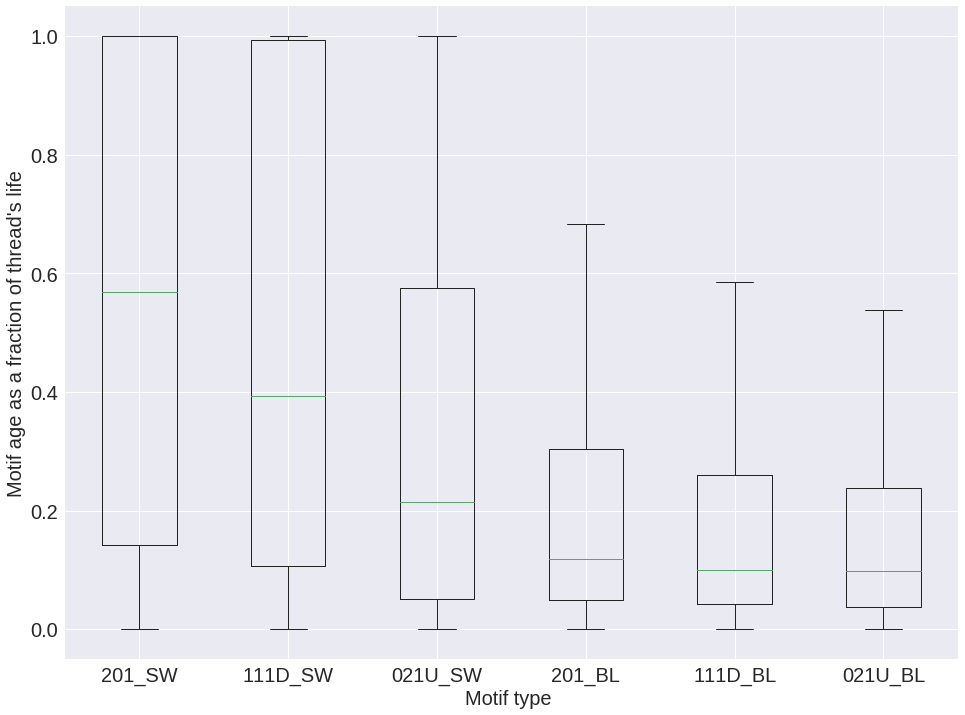
\includegraphics[width=0.5\textwidth, height = 6cm ]{Figures/BoxPlotMotifs_all.png}
		\label{fig:motifOccurance}
	}
	\subfloat[]{
		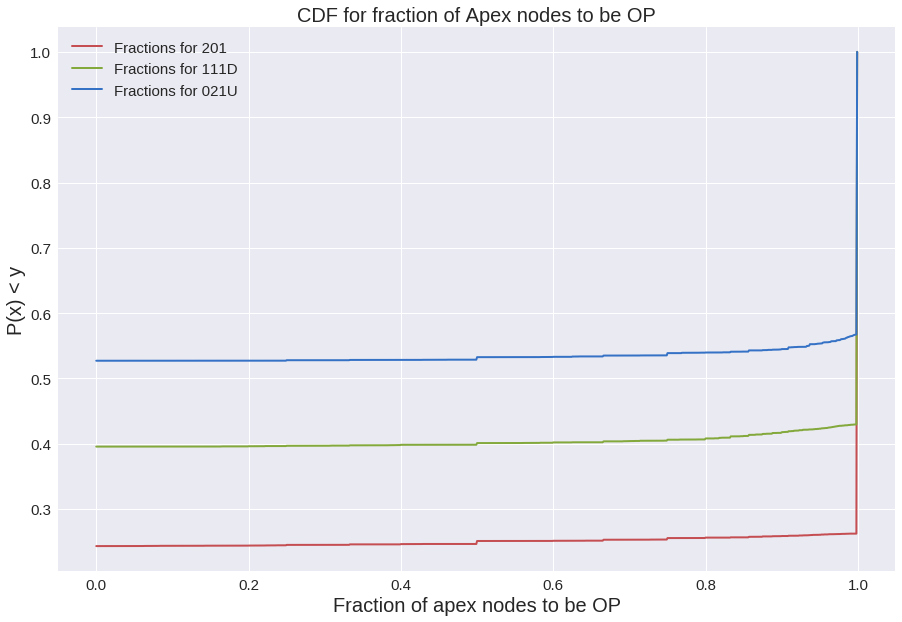
\includegraphics[width=0.5\linewidth, height = 6cm ]{Figures/CFD_ApexOP.png}
		\label{fig:ApexOPProp}
	}
    
    
\caption{This panel shows the statistical significance of the three over expressed and one under expressed triadic motif. Figure \ref{fig:motifOccurance} shows the distribution of each of the triadic motif's temporal point of occurrence according to the latest edge, as a proportion of the thread's lifetime. }
\end{figure}